\documentclass[journal]{IEEEtran}
\usepackage{graphicx}
\usepackage{amssymb,amsmath}

\begin{document}

\title{The Tor Network - Strengths and Weaknesses \\ \Large Computer Security 1 - CS5460 \\ \LaTeX{}}
\author{Jesse Victors \\ November 2013}

\maketitle

\section{Introduction}

The Tor network is a second-generation onion routing system that aims to provide anonymity, privacy, and Internet censorship protection to its users. Tour routes encrypted TCP traffic through a worldwide network of over four thousand relays run by volunteers across the world. Tor's encryption, authentication, and routing protocols are designed to make it infeasible for any adversary to identify an end user or reveal their traffic. Throughout its history, various organizations and governments have attempted to block, tap, or crack the Tor network. It was recently revealed that the US National Security Agency has attempted to penetrate the Tor network. Tor is also currently undergoing a transition from RSA-based to elliptic-curve-based TLS. In light of these attacks, Tor's popularity, and the protocol transition, a question that must be asked both by its users and by outsiders is: how secure is Tor? How does it work, what does it provide, and what are its weaknesses. In this paper, I address these questions.

\section{Design}

Tor provides an anonymity and privacy layer by relaying all end-user TCP traffic through a series of \textit{relays} on the Tor network. Typically this route consists of a carefully-constructed three-hop path known as a \textit{circuit}, which changes over time. These nodes in the circuit are referred to as \textit{entry guard}, \textit{middle router}, and the \textit{exit node}, respectively. Only the first node can determine the origin of TCP traffic through Tor, and only the exit node can examine the contents and its destination. Nodes in the middle are unable to determine either. No single node can determine the origin, the contents, and the destination of traffic through the network. Tor's architecture is designed to make it exceptionally difficult for a well-resourced adversary to uncover the identity of the end-user and their network activities, even if nodes are compromised.\cite{McCoy2008}

\subsection{Routing}

In traditional Internet connections, the client communicates directly with the server. In this model, an eavesdropper can often reveal both the identity of the end user and their activities. Direct encrypted connections do not hide IP headers, which expose source and destination addresses and the size of the payload. In the face of adversaries with sophisticated traffic analysis tools, such information can be very revealing for someone who wishes to hide their activities altogether.

Tor combats this by routing end user traffic through a randomized path through the network of relays. To construct this circuit, the Tor client software first queries a trusted directory server, which return a list of Tor nodes. This is illustrated in Figure 1.

\begin{figure}[htbp]
\centering
\begin{minipage}{8 cm}
    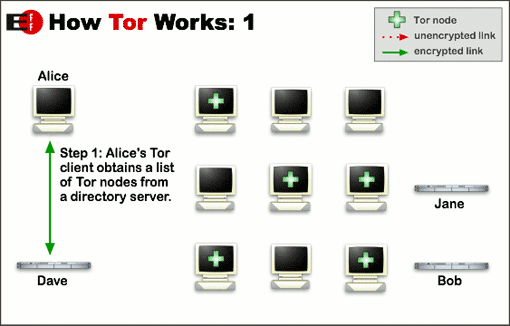
\includegraphics[width=80mm]{resources/circuit-building-1.png}
    \caption{The user's software first downloads a directory list of Tor relays. This information is later used to construct a circuit through the network.\cite{McCoy2008}}
\end{minipage}
\end{figure}

The second step involves choosing three nodes to use and carefully constructing an encrypted path between them. The circuit is extended one hop at a time such that no single relay ever knows the complete path. The client negotiates a separate set of encryption keys for each hop along the circuit to ensure that each hop cannot trace these connections as they pass through, as seen in Figure 2.

\begin{figure}[htbp]
\centering
\begin{minipage}{8 cm}
    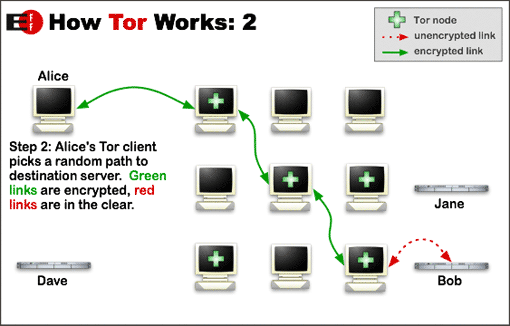
\includegraphics[width=80mm]{resources/circuit-building-2.png}
    \caption{A Tor circuit is incrementally constructed using layers of encryption. Each node has limited visibility, and no individual node knows the whole circuit.}
\end{minipage}
\end{figure}

Following the complete establishment of a circuit, TCP traffic can be routed through it. As each relay sees no more than one hop in the circuit, neither an eavesdropper nor a compromised relay can use traffic analysis to link the connection's source and destination. Tor further obfuscates user traffic by changing the circuit path every ten minutes,\cite{McCoy2008} as shown in Figure 3.

\begin{figure}[htbp]
\centering
\begin{minipage}{8 cm}
  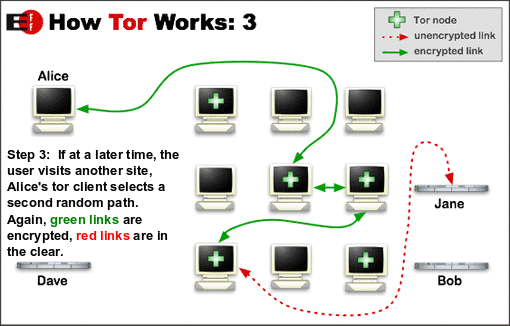
\includegraphics[width=80mm]{resources/circuit-building-3.png}
  \caption{A Tor circuit is changed periodically, essentially providing a new identity to the end user.}
\end{minipage}
\end{figure}

It should be noted that traffic exiting the Tor network is often (but not always) encrypted on its way to the source. An outsider is therefore faced with up to four layers of TLS encryption. Currently, Tor is one of the most secure tools to use against network surveillance, traffic analysis, and to bypassing information censorship.

\subsection{Encryption}

Encryption is a necessary component for privacy within the Tor network. Traffic passing between nodes must be secured from outsiders, and even compromised nodes must not be able to observe the traffic in cleartext. Privacy is also important for traffic outside the network; encrypted connections between the exit node and the target web server must also be achieved. Furthermore, two layers are needed: one for inside the network and one for outside it.

Within the network, nodes talk to each other via the Transport Security Layer (TLS) protocol. When a circuit is built, each pair of nodes within it must first come to an agreement over an encryption key and the specific cipher to use for encryption. There are several mechanisms by which this can be done, all of which use Diffie-Hellman (DH) for key exchange. The most common methods include: TLS\_RSA, which rely upon public and private keys generated with RSA; TLS\_DHE, ephemeral DH; TLS\_ECDH, DH based on elliptic curves, and TLS\_ECDHE, ephemeral elliptic curve DH. It should be noted that only TLS\_DHE and TLS\_ECDHE provide perfect forward secrecy, so it is no surprise that Tor exclusively prefers them. Once encryption keys and the specific cipher (as well as its mode) have been agreed upon, communication of traffic between two nodes can be encrypted and exchanged.

%http://security.stackexchange.com/questions/8343/what-key-exchange-mechanism-should-be-used-in-tls
%https://en.wikipedia.org/wiki/Comparison_of_TLS_implementations
%https://www.ipa.go.jp/security/rfc/RFC5246-ACJA.html
%4134 -- 0x0039 TLS_DHE_RSA - the key exchange is an ephemeral Diffie-Hellman: the server dynamically generates a DH public key and sends it to the client; the server also signs what it sends. For DHE_RSA, the server public key must be of type RSA, and its certificate must be appropriate for signatures (the Key Usage extension, if present, must include the digitalSignature flag).
%5566 -- 0xc013 TLS_ECDHE_RSA - the server sends a dynamically generated (ephemeral?) EC Diffie-Hellman key, and signs it with its own RSA key.

Tor users typically use the Tor Browser Bundle, (TBB) a custom build of Mozilla Firefox with a focus on security and pricacy. The TBB not only provides special handling of client-side scripts such as Javascript, but also offers the HTTPS Everywhere extension, which uses regular expressions to rewrite web requests into ones that use HTTPS. Thus, if the web server is capable of handling SSL or TLS connections, HTTP communications will be encrypted under them. Like any typical browser, the TBB negotiates with the web server for the cipher and keys required for SSL/TSL, except that this negotiation entirely occurs through the Tor circuit. As previously noted, this information, along with subsequent HTTP data, is encrypted between each node in the circuit. During transmission, each node in the circuit decrypts its layer in turn, until the final node (the exit) passes the data to the target server. The TLS/IP connections remain open, so the returned information likewise travels back up the circuit to the end user.

In September 2013, Robert Graham of Errata Security analyzed 22,920 incoming connections to his exit node and found that 89.9\; of the circuits agreed to use the Advanced Encryption Standard (AES) block cipher in cipher-block chaining (CBC) mode. This is the most common mode for AES, and allows for parallel decryption of the data blocks. The other 10.1\; of the circuits relied upon the Data Encryption Standard (DES) cipher for encryption. Furthermore, 75.7\% of the circuits used elliptic-curve DH, with the remaining 22.3\% relying upon traditional RSA DH.\cite{Graham2013} Both protocols are discussed below.

\subsubsection{RSA}

RSA is an algorithm for public-key cryptography. Its security is based on the infeasibility of factoring the product of two large primes. RSA, like all other public-key cryptography algorithms, relies upon two keys: one public and the other private. The public key may be published and is used for encryption and for verifying digital signatures. The private key is used for decryption, the generation of digital signatures. Thus, through RSA, only the owner of the private key can decrypt incoming messages, and only they can digitally sign outbound messages. This makes RSA extremely powerful for both authenticity and privacy.

To generate the RSA keys, two distinct prime numbers of similar bit-length are chosen at random, \textit{p} and \textit{q}. \textit{n} is computed as the product of \textit{p} and \textit{q}, and it is used as the modulus for both the public and private keys. The bit-length of \textit{n} is the RSA key length. Then let φ(n)\; =\; φ(p) φ(q)\; =\; (p − 1) (q − 1)\; where φ is Euler's totient function, which counts the number of positive integers less than or equal to \textit{n} that are relatively prime to \textit{n}. Then \textit{e} is chosen such that \textit{e} and φ(n) are coprime. \textit{d} is also chosen such that it is the multiplicative inverse of e modulo φ(n). The RSA public key then consists of the modulus \textit{n} and the exponent \textit{e}. The private key likewise consists of \textit{n} and the exponent \textit{d}.

A message \textit{M} is encrypted by first blocks of length less than \textit{n} using an agreed-upon padding scheme. The ciphertext \textit{c} is then computed as m\^e mod n, which can be calculated quickly using the method of exponentiation by squaring. The recipient (the owner of the private key) can then recover the plaintext \textit{M} by computing c\^d mod n, and then reversing the padding scheme. The decryption process is often accelerated by optimizations such as the Chinese Remainder Theorem. Furthermore, to sign a message, the owner of the private key first uses an agreed-upon hash function to compute a hash value of the message, raises it to the power of \textit{d} modulo \textit{n} and then sends that in conjuction with \textit{M}. The recipient, who only has access to the public keys, then raises the signature to the power of \textit{e} modulo \textit{n} and compares the result with his hash of the message using the same hash algorithm. If the two match, then he can prove the authenticity and integrity of the message. These two capabilities make RSA an extremely powerful tool for securing authenticity, integrity, and privacy of communication between two parties.

\subsubsection{Elliptic-curve}

Elliptic Curve Cryptography (ECC) is an approach to public-key cryptography in which elliptic curves are used instead of RSA. In contrast to RSA, ECC relies upon the infeasiblity of finding the discrete logarithm of a random elliptic curve element with respect to a publicly known base point. This is known as the elliptic curve discrete logarithm problem, or ECDLP.

Elliptic curves over the real number system can be defined through the equation,
y\^2\; =\; x\^3\; +\; a x\; +\; b\;
Where \textit{a} and \textit{b} are real numbers. This formula describes a plane curve through the Euclidean plane, although elliptic curves do exists in other spaces. However, current cryptographic purposes only work with elliptic curves within the context of the real number systems.

A smaller key size is one of the most significant benefits introduced by ECC. Current NIST recommendations state that a key size of 160 bits for ECC offers a similar level of security to 1024 bits of RSA/DH. Likewise, 224 bits for ECC is analogous to 2048 bits of RSA/DH. It should be noted that the required key sizes for ECC increases significantly slower than the key sizes for RSA and Diffie-Hellman increase at a much faster rate than the required key size for ECC. Thus ECC offers more security per increase in key size than for RSA. The smaller key size also directly correlates to an increase in computational efficiency; as the bit size increases, the speed difference between Diffie-Hellman and ECC grows superlinearly.\cite{CaseForECC}

Tor 2.4.x introduced ECC into its DH key exchange protocols, known as \textit{NTor}.

\subsection{Authentication}

Authentication...

\section{Features}

\subsection{SOCKS}

The Tor client software offers a Secure Sockets (SOCKS) interface on the system's localhost. SOCKS is different than HTTP proxying, although it uses handshake protocols for authorization purposes, it does not interpret or rewrite any of the subsequent traffic. The Tor Browser Bundle uses this interface as an input to the Tor network, although other applications may also utilize it. SOCKS then multiplexes traffic through the Tor circuit.

\subsection{Hidden services}

% https://en.wikipedia.org/wiki/Core.onion
% https://en.wikipedia.org/wiki/DuckDuckGo
% https://en.wikipedia.org/wiki/The_Hidden_Wiki
% https://www.torproject.org/docs/hidden-services.html.en

\section{Adversaries}

It was recently revealed that the National Security Administration (NSA) has been targeting Tor, albeit with marginal success in breaking the anonymity and privacy of its users. However, in early October, the FBI successfully identified and arrested the owner of the Silk Road, a black market operating as a hidden service within the Tor network, and seized the service.

\section{Challenges}

TBB - javascript and cross-scripting
Does the web server support SSL/TLS?

To achieve its low-latency objective, Tor does not explicitly re-order or delay packets within the network.\cite{McCoy2008}

% https://en.wikibooks.org/wiki/LaTeX/Bibliography_Management
\begin{thebibliography}{9}

% http://homes.cs.washington.edu/~yoshi/papers/Tor/PETS2008_37.pdf
\bibitem{McCoy2008}
  Damon McCoy, Kevin Bauer, Dirk Grunwald, Tadayoshi Kohno, Douglas Sicker,
  \emph{Shining Light in Dark Places: Understanding the Tor Network}.
  Department of Computer Science and Engineering,
  University of Washington, Seattle, WA 98195-2969,
  2008.

% http://delivery.acm.org/10.1145/1320000/1314336/p11-bauer.pdf?ip=129.123.212.2&id=1314336&acc=ACTIVE%20SERVICE&key=C2716FEBFA981EF14CED21A2601DAAECFD63F9AFA4F38248&CFID=375634674&CFTOKEN=21383502&__acm__=1383519744_1cd525050cafbe9ffe083b269ff783d9
\bibitem{Bauer2007}
  Kevin Bauer, Damon McCoy, Dirk Grunwald, Tadayoshi Kohno, Douglas Sicker
  \emph{Low-resource routing attacks against tor}.
  ACM, 2007

% http://ieeexplore.ieee.org/stamp/stamp.jsp?tp=&arnumber=5636000&tag=1
\bibitem{Chaabane2007}
  Abdelberi Chaabane, Pere Manils, Mohamed Ali Kaafar
  \emph{Digging into Anonymous Traffic: a deep analysis of the Tor anonymizing network}.
  IEEE, 2010

% https://www.torproject.org/docs/faq.html.en
\bibitem{TorFAQ}
  Tor FAQ

% http://www.nsa.gov/business/programs/elliptic_curve.shtml
\bibitem{CaseForECC}
  National Security Agency
  \emph{The Case for Elliptic Curve Cryptography}.
  NSA, 2009

% http://blog.erratasec.com/2013/09/tor-is-still-dhe-1024-nsa-crackable.html
% http://thehackernews.com/2013/09/NSA-can-crack-TOR-Encryptio-Snowden-files-.html
\bibitem{Graham2013}
  Robert Graham
  \emph{Tor is still DHE 1024 (NSA crackable)}.
  Errata Security, 2013

\end{thebibliography}

\end{document}
